\documentclass[11pt,oneside]{article}
\usepackage[T1]{fontenc}
\usepackage[utf8]{inputenc}
% \usepackage{lmodern}
%\usepackage[adobe-utopia,uppercase=upright,greeklowercase=upright]{mathdesign}
\usepackage[adobe-utopia]{mathdesign}
%\usepackage{minionpro}
% \usepackage{pifont}
% \usepackage{amssymb}
\usepackage{amsmath}
\usepackage[francais]{babel}
% \usepackage[francais]{varioref}
\usepackage[dvips]{graphicx}

\usepackage{framed}
\usepackage[normalem]{ulem}
\usepackage{fancyhdr}
\usepackage{titlesec}
\usepackage{vmargin}
\usepackage{longtable}

\usepackage{ifthen}


%\usepackage{epsfig}
\usepackage{subfig}

\usepackage{multirow}
\usepackage{multicol} % Portions de texte en colonnes
\usepackage{flafter}%floatants après la référence



\usepackage{color}
\usepackage{colortbl}


\definecolor{gris25}{gray}{0.75}
\definecolor{bleu}{RGB}{18,33,98}
\definecolor{bleuf}{RGB}{42,94,171}
\definecolor{bleuc}{RGB}{231,239,247}
\definecolor{rougef}{RGB}{185,18,27}
\definecolor{rougec}{RGB}{255,230,231}
\definecolor{vertf}{RGB}{103,126,82}
\definecolor{vertc}{RGB}{220,255,191}

\newenvironment{rem}[1][\hsize]%
{%
    \def\FrameCommand
    {%
\rotatebox{90}{\textit{\textsf{Remarque}}} 
        {\color{bleuf}\vrule width 3pt}%
        \hspace{0pt}%must no space.
        \fboxsep=\FrameSep\colorbox{bleuc}%
    }%
    \MakeFramed{\hsize#1\advance\hsize-\width\FrameRestore}%
}%
{\endMakeFramed}%


\newenvironment{savoir}[1][\hsize]%
{%
    \def\FrameCommand
    {%
\rotatebox{90}{\textit{\textsf{Savoir}}} 
        {\color{bleuf}\vrule width 3pt}%
        \hspace{0pt}%must no space.
        \fboxsep=\FrameSep\colorbox{bleuc}%
    }%
    \MakeFramed{\hsize#1\advance\hsize-\width\FrameRestore}%
}%
{\endMakeFramed}%

\newenvironment{prob}[1][\hsize]%
{%
    \def\FrameCommand%
    {%
\rotatebox{90}{\textit{\textsf{ Problématique}}} 
        {\color{rougef}\vrule width 3pt}%
        \hspace{0pt}%must no space.
        \fboxsep=\FrameSep\colorbox{rougec}%
    }%
    \MakeFramed{\hsize#1\advance\hsize-\width\FrameRestore}%
}%
{\endMakeFramed}%

\newenvironment{obj}[1][\hsize]%
{%
    \def\FrameCommand%
    {%
\rotatebox{90}{\textit{\textsf{ $\;$}}} 
        {\color{rougef}\vrule width 3pt}%
        \hspace{0pt}%must no space.
        \fboxsep=\FrameSep\colorbox{rougec}%
    }%
    \MakeFramed{\hsize#1\advance\hsize-\width\FrameRestore}%
}%
{\endMakeFramed}%

\newenvironment{defi}[1][\hsize]%
{%
    \def\FrameCommand%
    {%
\rotatebox{90}{\textit{\textsf{Définition\\}}} 
        {\color{bleuf}\vrule width 3pt}%
        \hspace{0pt}%must no space.
        \fboxsep=\FrameSep\colorbox{bleuc}%
    }%
    \MakeFramed{\hsize#1\advance\hsize-\width\FrameRestore}%
}%
{\endMakeFramed}%


\newenvironment{hypo}[1][\hsize]%
{%
    \def\FrameCommand%
    {%
\rotatebox{90}{\textit{\textsf{Hypothèse\\}}} 
        {\color{bleuf}\vrule width 3pt}%
        \hspace{0pt}%must no space.
        \fboxsep=\FrameSep\colorbox{bleuc}%
    }%
    \MakeFramed{\hsize#1\advance\hsize-\width\FrameRestore}%
}%
{\endMakeFramed}%


\newenvironment{prop}[1][\hsize]%
{%
    \def\FrameCommand%
    {%
\rotatebox{90}{\textit{\textsf{Propriété\\}}} 
        {\color{bleuf}\vrule width 3pt}%
        \hspace{0pt}%must no space.
        \fboxsep=\FrameSep\colorbox{bleuc}%
    }%
    \MakeFramed{\hsize#1\advance\hsize-\width\FrameRestore}%
}%
{\endMakeFramed}%

\newenvironment{props}[1][\hsize]%
{%
    \def\FrameCommand%
    {%
\rotatebox{90}{\textit{\textsf{Propriétés\\}}} 
        {\color{bleuf}\vrule width 3pt}%
        \hspace{0pt}%must no space.
        \fboxsep=\FrameSep\colorbox{bleuc}%
    }%
    \MakeFramed{\hsize#1\advance\hsize-\width\FrameRestore}%
}%
{\endMakeFramed}%

\newenvironment{exemple}[1][\hsize]%
{%
    \def\FrameCommand%
    {%
\rotatebox{90}{\textit{\textsf{Exemple\\}}} 
        {\color{vertf}\vrule width 3pt}%
        \hspace{0pt}%must no space.
        \fboxsep=\FrameSep\colorbox{vertc}%
    }%
    \MakeFramed{\hsize#1\advance\hsize-\width\FrameRestore}%
}%
{\endMakeFramed}%

\newenvironment{resultat}[1][\hsize]%
{%
    \def\FrameCommand%
    {%
\rotatebox{90}{\textit{\textsf{Résultat\\}}} 
        {\color{rougef}\vrule width 3pt}%
        \hspace{0pt}%must no space.
        \fboxsep=\FrameSep\colorbox{rougec}%
    }%
    \MakeFramed{\hsize#1\advance\hsize-\width\FrameRestore}%
}%
{\endMakeFramed}%

\newenvironment{methode}[1][\hsize]%
{%
    \def\FrameCommand%
    {%
\rotatebox{90}{\textit{\textsf{Méthode\\}}} 
        {\color{rougef}\vrule width 3pt}%
        \hspace{0pt}%must no space.
        \fboxsep=\FrameSep\colorbox{rougec}%
    }%
    \MakeFramed{\hsize#1\advance\hsize-\width\FrameRestore}%
}%
{\endMakeFramed}%

\newenvironment{theo}[1][\hsize]%
{%
    \def\FrameCommand%
    {%
\rotatebox{90}{\textit{\textsf{Théorème\\}}} 
        {\color{rougef}\vrule width 3pt}%
        \hspace{0pt}%must no space.
        \fboxsep=\FrameSep\colorbox{rougec}%
    }%
    \MakeFramed{\hsize#1\advance\hsize-\width\FrameRestore}%
}%
{\endMakeFramed}%

\newenvironment{warn}[1][\hsize]%
{%
    \def\FrameCommand%
    {%
\rotatebox{90}{\textit{\textsf{Attention\\}}} 
        {\color{rougef}\vrule width 3pt}%
        \hspace{0pt}%must no space.
        \fboxsep=\FrameSep\colorbox{rougec}%
    }%
    \MakeFramed{\hsize#1\advance\hsize-\width\FrameRestore}%
}%
{\endMakeFramed}%

% \usepackage{pstricks}
%\usepackage{minitoc}
% \setcounter{minitocdepth}{4}

\setcounter{tocdepth}{2}

% \mtcselectlanguage{french} 

%\usepackage{draftcopy}% "Brouillon"
% \usepackage{floatflt}
\usepackage{psfrag}
%\usepackage{listings} % Permet d'insérer du code de programmation
\renewcommand{\baselinestretch}{1.2}

% Changer la numérotation des figures :
% ------------------------------------
% \makeatletter
% \renewcommand{\thefigure}{\ifnum \c@section>\z@ \thesection.\fi
%  \@arabic\c@figure}
% \@addtoreset{figure}{section}
% \makeatother
 


%%%%%%%%%%%%
% Définition des vecteurs %
%%%%%%%%%%%%
 \newcommand{\vect}[1]{\overrightarrow{#1}}

%%%%%%%%%%%%
% Définition des torseusr %
%%%%%%%%%%%%

 \newcommand{\torseur}[1]{%
\left\{{#1}\right\}
}

\newcommand{\torseurcin}[3]{%
\left\{\mathcal{#1} \left(#2/#3 \right) \right\}
}

\newcommand{\torseurstat}[3]{%
\left\{\mathcal{#1} \left(#2\rightarrow #3 \right) \right\}
}

 \newcommand{\torseurc}[8]{%
%\left\{#1 \right\}=
\left\{
{#1}
\right\}
 = 
\left\{%
\begin{array}{cc}%
{#2} & {#5}\\%
{#3} & {#6}\\%
{#4} & {#7}\\%
\end{array}%
\right\}_{#8}%
}

 \newcommand{\torseurcol}[7]{
\left\{%
\begin{array}{cc}%
{#1} & {#4}\\%
{#2} & {#5}\\%
{#3} & {#6}\\%
\end{array}%
\right\}_{#7}%
}

 \newcommand{\torseurl}[3]{%
%\left\{\mathcal{#1}\right\}_{#2}=%
\left\{%
\begin{array}{l}%
{#1} \\%
{#2} %
\end{array}%
\right\}_{#3}%
}

 \newcommand{\vectv}[3]{%
\vect{V\left( {#1} \in {#2}/{#3}\right)}
}


\newcommand{\vectf}[2]{%
\vect{R\left( {#1} \rightarrow {#2}\right)}
}

\newcommand{\vectm}[3]{%
\vect{\mathcal{M}\left( {#1}, {#2} \rightarrow {#3}\right)}
}


 \newcommand{\vectg}[3]{%
\vect{\Gamma \left( {#1} \in {#2}/{#3}\right)}
}

 \newcommand{\vecto}[2]{%
\vect{\Omega\left( {#1}/{#2}\right)}
}
% }$$\left\{\mathcal{#1} \right\}_{#2} =%
% \left\{%
% \begin{array}{c}%
%  #3 \\%
%  #4 %
% \end{array}%
% \right\}_{#5}}

%  ------------------------------------------
% | Modification du formatage des sections : | 
%  ------------------------------------------

% Grands titres :
% ---------------

\newcommand{\titre}[1]{%
\begin{center}
      \bigskip
      \rule{\textwidth}{1pt}
      \par\vspace{0.1cm}
      
      \textbf{\large #1}
      \par\rule{\textwidth}{1pt}
    \end{center}
    \bigskip
  }

% Supprime le numéro du chapitre dans la numérotation des sections:
% -----------------------------------------------------------------
\makeatletter
\renewcommand{\thesection}{\@arabic\c@section}
\makeatother


% \titleformat{\chapter}[display]
% {\normalfont\Large\filcenter}
% {}
% {1pc}
% {\titlerule[1pt]
%   \vspace{1pc}%
%   \Huge}[\vspace{1ex}%
% \titlerule]


%%%% Chapitres Comme PY Pechard %%%%%%%%%
% numéro du chapitre
\DeclareFixedFont{\chapnumfont}{OT1}{phv}{b}{n}{80pt}
% pour le mot « Chapitre »
\DeclareFixedFont{\chapchapfont}{OT1}{phv}{m}{it}{40pt}
% pour le titre
\DeclareFixedFont{\chaptitfont}{T1}{phv}{b}{n}{25pt}

\definecolor{gris}{gray}{0.75}
\titleformat{\chapter}[display]%
	{\sffamily}%
	{\filleft\chapchapfont\color{gris}\chaptertitlename\
	\\
	\vspace{12pt}
	\chapnumfont\thechapter}%
	{16pt}%
	{\filleft\chaptitfont}%
	[\vspace{6pt}\titlerule\titlerule\titlerule]

%%%%  Fin Chapitres Comme PY Pechard %%%%%%%%%


% Section, subsection, subsubsection sans serifs :
% % ----------------------------------------------

% \makeatletter
% \renewcommand{\section}{\@startsection{section}{0}{0mm}%
% {\baselineskip}{.3\baselineskip}%
% {\normalfont\sffamily\Large\textbf}}%
% \makeatother

\makeatletter
\renewcommand{\@seccntformat}[1]{{\textcolor{bleu}{\csname
the#1\endcsname}\hspace{0.5em}}}
\makeatother

\makeatletter
\renewcommand{\section}{\@startsection{section}{1}{\z@}%
                       {-4ex \@plus -1ex \@minus -.4ex}%
                       {1ex \@plus.2ex }%
                       {\normalfont\Large\sffamily\bfseries}}%
\makeatother
 
\makeatletter
\renewcommand{\subsection}{\@startsection {subsection}{2}{\z@}
                          {-3ex \@plus -0.1ex \@minus -.4ex}%
                          {0.5ex \@plus.2ex }%
                          {\normalfont\large\sffamily\bfseries}}
\makeatother
 
\makeatletter
\renewcommand{\subsubsection}{\@startsection {subsubsection}{3}{\z@}
                          {-2ex \@plus -0.1ex \@minus -.2ex}%
                          {0.2ex \@plus.2ex }%
                          {\normalfont\large\sffamily\bfseries}}
\makeatother
 
\makeatletter             
\renewcommand{\paragraph}{\@startsection{paragraph}{4}{\z@}%
                                    {-2ex \@plus-.2ex \@minus .2ex}%
                                    {0.1ex}%               
{\normalfont\sffamily\bfseries}}
\makeatother
 
\makeatletter
\renewcommand{\subparagraph}{\@startsection{subparagraph}{5}{\z@}%
                                       {-2ex \@plus-.1ex \@minus .2ex}%
                                       {0.1ex}%
				    {\normalfont\normalsize\sffamily\bfseries}}
\makeatletter
% \makeatletter
% \renewcommand{\subsection}{\@startsection{subsection}{1}{2mm}%
% {\baselineskip}{.3\baselineskip}%
% {\normalfont\sffamily\large\textbf}}%
% \makeatother
% 
% \makeatletter
% \renewcommand{\subsubsection}{\@startsection{subsubsection}{2}{4mm}%
% {\baselineskip}{.15\baselineskip}%
% {\normalfont\sffamily\large\textbf}}%
% \makeatother
% 
% \makeatletter
% \renewcommand{\paragraph}{\@startsection{paragraph}{3}{6mm}%
% {\baselineskip}{.15\baselineskip}%
% {\normalfont\sffamily\large\textbf}}%
% \makeatother
 
\setcounter{secnumdepth}{4}


%  --------
% | Marges |
%  --------


% \setmarginsrb{2.5cm}{1.5cm}{2.5cm}{2cm}{1cm}{1cm}{1cm}{1cm}
\setmarginsrb{1.5cm}{1cm}{1cm}{1.5cm}{1cm}{1cm}{1cm}{1cm}

% Changer les marges localement :
% -----------------------------
\newenvironment{changemargin}[2]{\begin{list}{}{%
\setlength{\topsep}{0pt}%
\setlength{\leftmargin}{0pt}%
\setlength{\rightmargin}{0pt}%
\setlength{\listparindent}{\parindent}%
\setlength{\itemindent}{\parindent}%
\setlength{\parsep}{0pt plus 1pt}%
\addtolength{\leftmargin}{#1}%
\addtolength{\rightmargin}{#2}%
}\item }{\end{list}}



\usepackage{pst-solides3d}
\usepackage{titletoc}
\titlecontents{chapter}[+3pc]
  {\addvspace{10pt}\sffamily\bfseries}
{\contentslabel[{\pscirclebox[fillstyle=solid,fillcolor=gray!25,
linecolor=gray!25,framesep=4pt]{\textcolor{white}{\thecontentslabel}}}]{2.5pc}}
  {}
  {\dotfill \normalfont\thecontentspage\ }

\titlecontents{section}[3pc]
  {\addvspace{2pt}\sffamily}
  {\contentslabel[\thecontentslabel]{1.8pc}}
  {}
  {\dotfill \normalfont\thecontentspage\ }

\titlecontents{subsection}[5pc]
  {\addvspace{2pt}\sffamily}
  {\contentslabel[\thecontentslabel]{1.8pc}}
  {}
  {\dotfill \normalfont\thecontentspage\ }

\titlecontents{subsubsection}[8pc]
  {\addvspace{2pt}\sffamily}
  {\contentslabel[\thecontentslabel]{3pc}}
  {}
  {\dotfill \normalfont\thecontentspage\ }
%{\;\titlerule\;\normalfont\thecontentspage\ }

\titlecontents{paragraph}[9pc]
  {\addvspace{2pt}\sffamily}
  {\contentslabel[\thecontentslabel]{3.5pc}}
  {}
  {\dotfill \normalfont\thecontentspage\ }




\usepackage[%
    pdftitle={DM5 - Cinématique},
    pdfauthor={Xavier Pessoles},
    colorlinks=true,
    linkcolor=blue,
    citecolor=magenta]{hyperref}

\usepackage{schemabloc}

% \makeatletter \let\ps@plain\ps@empty \makeatother
%% DEBUT DU DOCUMENT
%% =================
\sloppy
\hyphenpenalty 10000



\colorlet{shadecolor}{orange!15}

\begin{document}


\newboolean{prof}
\setboolean{prof}{true}
%------------- En tetes et Pieds de Pages ------------
\pagestyle{fancy}
\renewcommand{\headrulewidth}{0pt}

\fancyhead{}
\fancyhead[L]{%
\begin{minipage}[c]{1.6cm}

\includegraphics[width=2cm]{png/logo_ptsi.png}%
\end{minipage}
\rule{2cm}{.5pt}
}

\fancyhead[C]{\rule{11cm}{.5pt}}

\fancyhead[R]{%
\begin{minipage}[c]{3cm}
\begin{flushright}
\footnotesize{\textit{\textsf{Sciences Industrielles\\ de l'Ingénieur}}}%
\end{flushright}
\end{minipage}
}

\renewcommand{\footrulewidth}{0.2pt}

\fancyfoot[C]{\footnotesize{\bfseries \thepage}}
\fancyfoot[L]{\footnotesize{2012 -- 2013} \\ X. \textsc{Pessoles}}
\ifthenelse{\boolean{prof}}{%
\fancyfoot[R]{\footnotesize{DM 7}}
}{%
\fancyfoot[R]{\footnotesize{DM 6}}%-- CI 3 : Statique \& CI 6 : PPM}}
}


%\begin{center}
%\textit{Centre d'intérêt}
%\end{center}

\begin{center}
 \Large\textsc{Devoir Maison 7}
\end{center}

\begin{center}
 \large\textsc{A rendre le mercredi 6 février 2013} 
\end{center}


\vspace{0.5cm}


\noindent\rule{\linewidth}{.2pt}
\begin{center}
 %\large\textbf{CI 4} \textit{Conception des mécanismes}

 \large\textbf{CI 5} \textit{Communication technique : Schémas et géométrie des pièces, architecture des systèmes pluritechniques}
\end{center}
\noindent\rule{\linewidth}{.2pt}


\vspace{0.5cm}




\noindent\rule{\linewidth}{.2pt}
\begin{center}
 \LARGE\textbf{\textsc{Boîte de transfert de 4x4}}
\end{center}
\noindent\rule{\linewidth}{.2pt}



\section{Étude préliminaire -- Analyse du besoin}

On s'intéresse à la figure située sur le document réponse faisant référence à la figure 2 présent sur le document 1 (dessin d'ensemble). Cette figure présente un véhicule automobile en phase de virage. La vitesse de déplacement du véhicule est connue au point $M$. $\vectv{M}{1}{sol}$ est dirigée suivant $\vect{x}$.

L'angle de virage de la roue droite par rapport à la direction $\vect{z}$ vaut $\alpha_D$. La roue droite est considérée comme motrice. En conséquence, $\vectv{D}{1}{Sol}$ a la même direction que la roue avant droite. 

\paragraph{}
\textit{Déterminer l'angle de rotation de la roue gauche $\alpha_G$ du véhicule en fonction de $\alpha_D$, de l'empattement $e$ et de la voie $v$. L'empattement $e$ est la distance $DC$ entre les essieux avant et arrière. La voie $v$ est la distance $DG$ entre le centre des deux roues.}



\paragraph{}
\textit{Proposer un schéma cinématique minimal, à main levée, permettant de prendre en compte que les deux roues ne tournent pas du même angle lors d'un virage. }


\paragraph{}
\textit{On donne $||\vectv{M}{1}{sol}||=30\; km/h$. L'angle de rotation de la roue droite est de $45\degres$. Déterminer graphiquement, sur le schéma en fin de document, la vitesse aux points $B$, $C$, $D$ et $G$. Que peut-on en conclure ?}


\paragraph{}
\textit{Tracer le champ des vecteurs vitesses sur une largeur de pneu lors d'un virage. Que peut-on en conclure ?}



\paragraph{}
\textit{En utilisant une bête à cornes, dire à quel besoin devra répondre la boîte de transfert du 4x4.}


\section{Boîte de transfert}

\subsection{Fonctionnement}

Sur un véhicule de type 4x4, le mouvement de rotation du moteur est transmis à une boîte de vitesse commandée manuellement par un levier permettant de commander 5 rapports de vitesse ainsi que la marche arrière. En sortie de boîte de vitesse, la mouvement de rotation est transmis à l'arbre \textbf{4} de la boîte de transfert. 

\begin{center}
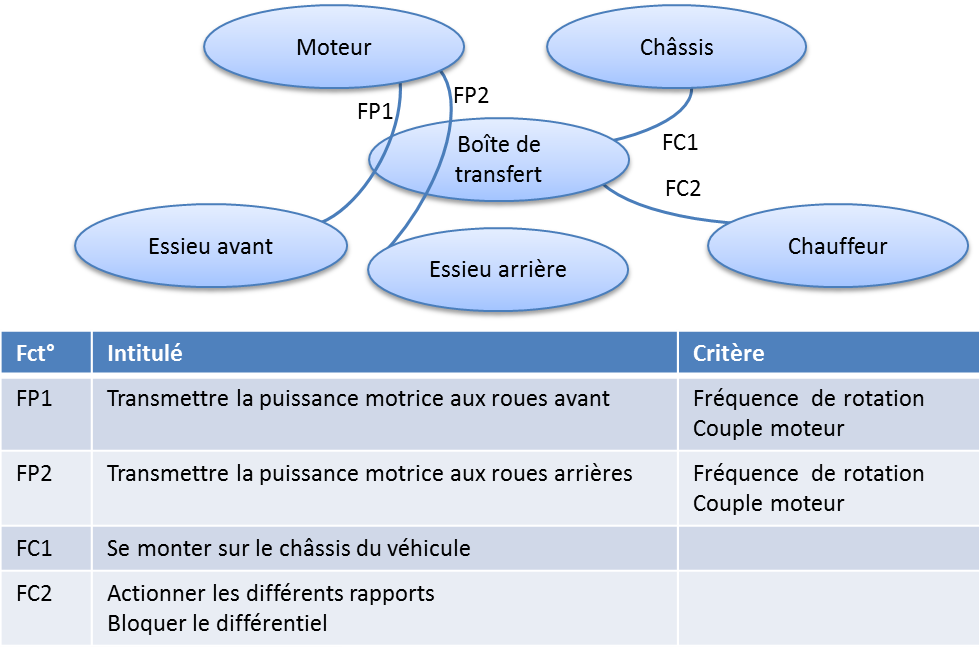
\includegraphics[width=.85\textwidth]{png/af}
\end{center}

La boîte de transfert comporte 2 rapports de vitesses commandée par le levier  \textbf{V2}: 
\begin{itemize}
\item un premier rapport utilisé sur route qui utilise les pignons 1 et 5;
\item un second rapport utilisé en tout-terrain qui utilise les pignons 3 ainsi que l'engrenage taillé sur l'arbre 6.
\end{itemize}

En sortie de la boîte de transfert, le mouvement est transmis vers les essieux avant et arrière. 

Un différentiel composé d'un train épicycloïdal est incorporé à cette boîte de transfert. Il permet aux essieux avant et arrières de tourner à des vitesses différentes. 

En actionnant le levier \textbf{D} il est possible de bloquer le différentiel. Les essieux avant et arrières tournent alors à la même vitesse. 

\subsection{Étude technologique}


\paragraph{}
\textit{D'après vous, comment est assurée la lubrification du système ? Comment est assurée la vidange ? Comment est assurée l'étanchéité vis-à-vis du milieu extérieur. }

\paragraph{}
\textit{Citer les 4 différentes technologies de roulements présentes dans la boîte de transfert. Indiquer leurs particularités et leurs cas d'utilisation.}

\paragraph{}
\textit{On dénote un jeu entre la bague extérieure du roulement \textbf{32} et le flasque \textbf{30} ainsi que la carter \textbf{33}. Quel est son but ?}

\paragraph{}
\textit{Proposer un matériau pour l'arbre \textbf{6}. Comment a-t-il été fabriqué ?}
%
%L'arbre va transmettre la totalité de la puissance du moteur aux différents essieux (au rendement près). C'est donc une pièce très forte sollicitée mécaniquement.
%
%On peut donc utiliser un acier, par exemple un $42 \; Cr\; Mo \; 4$. 
%
%\'A partir d'un brut laminé, on va forger la préforme de l'arbre. Les opérations suivantes vont être réalisées en tournage : 
%\begin{itemize}
%\item chariotage des cylindres;
%\item dressage de la face; 
%\item usinage des gorges,
%\item réalisation des filetages
%\end{itemize}
%
%La rainure de clavette sera usinée en fraisage (fraise 2 tailles). Enfin, les dents seront taillées par mortaisage (avec pignon ou crémaillère).
%
%(Des traitements thermiques seront certainement aussi réalisés).

\paragraph{}
\textit{Un palier lisse est présent entre l'arbre \textbf{9} et la pièce \textbf{25}. Quel est son but ? Proposer un matériau ? Comment a-t-il été fabriqué ?}

\subsection{Étude cinématique}

\paragraph{}
\textit{Identifiez les différentes classes d'ensemble cinématique en coloriant le dessin d'ensemble. On précise que les pièces \textbf{10} (couronne à denture intérieure), \textbf{11}  (pignon - satellite), \textbf{9} (pignon - planétaire) et \textbf{25} (porte-satellite) forment un train épicycloïdal\footnote{Seules les pièces principales des classes d'équivalences cinématiques sont citées.}.}


\paragraph{}
\textit{Quelle pièce permet le passage de la vitesse "route" à la vitesse 4x4" via le levier \textbf{V2} ? Quel est le mouvement de cette pièce ? Comment est-elle mise en mouvement ? Expliquer comment elle permet de sélectionner chacune des deux vitesses. Vous pourrez éventuellement vous aider de schémas.}

\paragraph{}
\textit{Quelle influence a le levier \textbf{D} sur le fonctionnement de la boîte de transfert ?}


\paragraph{}
\textit{En vous aidant des croquis présents sur le dessin d'ensemble, tracer le schéma cinématique minimal de la boîte de transfert. Vous pourrez utiliser le schéma cinématique du train épicycloïdal donné en fin de document en l'adaptant à notre cas.}


\paragraph{}
\textit{Déterminer les deux rapports de vitesse permis par la boîte de transfert.}

On donne $d_1 = d_{13} = 86\; mm$, $d_3=54\; mm$, $d_5=56\; mm$, $d_6=88\; mm$.


\subsection{Étude du train épicycloïdal}

\paragraph{}
\textit{Tracer le schéma cinématique du train épicycloïdal. Mettre en évidence par des figures planes, les vecteurs instantanés de rotations suivants :
\begin{itemize}
\item  rotation de l'arbre d'entrée du train (porte-satellite) par rapport au bâti : $\vecto{13}{33}$; 
\item  rotation de l'arbre essieu avant par rapport au bâti : $\vecto{9}{33}$; 
\item  rotation de l'arbre essieu arrière par rapport au bâti : $\vecto{10}{33}$; 
\item  rotation du satellite par rapport au porte-satellite : $\vecto{11}{13}$.
\end{itemize}
Vous indiquerez les centres des liaisons ainsi que les points de contacts entre les engrenages. Chacun de ces points pourront être ramenés dans un seul plan. Lors du fonctionnement du train épicycloïdal, ces points seront toujours alignés sur suivant le porte-satellite \textbf{13}.
}

\paragraph{}
\textit{Tracer le graphe des liaisons associé au train épicycloïdal.}

\paragraph{}
\textit{Après avoir écrit la relation de roulement sans glissement entre \textbf{10} et \textbf{11}, décomposer le vecteur vitesse pour obtenir une relation entre : $R_{10}$, $R_{11}$, $\omega_{10/33}$, $\omega_{13/11}$ et $\omega_{13/33}$.}

\paragraph{}
\textit{Après avoir écrit la relation de roulement sans glissement entre \textbf{11} et \textbf{9}, décomposer le vecteur vitesse pour obtenir une relation entre : $R_9$, $R_{11}$, $\omega_{9/33}$ et $\omega_{13/11}$ et $\omega_{13/33}$.}

\paragraph{}
\textit{Déterminer une relation géométrique permettant de lier $R_{9}$, $R_{11}$ et $R_{10}$.}

\paragraph{}
\textit{A partir des 3 relations précédentes, montrer que : 
$$
\dfrac{5}{3}\omega_{(12/33)} = \omega_{(10/33)}+\omega_{(9/33)}
$$
On donne : $R_{10}=42\;mm$, $R_{9}=21\;mm$, $R_{11}=10,5 \;mm$.}

\paragraph{}
\textit{Que se passe-t-il si le train avant est bloqué dans un obstacle ?}



\paragraph{}
\textit{Que se passe-t-il si le train arrière est bloqué dans un obstacle ?}

\paragraph{}
\textit{Que se passe-t-il si lorsque le différentiel est bloqué ?}

\vspace{2cm}

\begin{center}
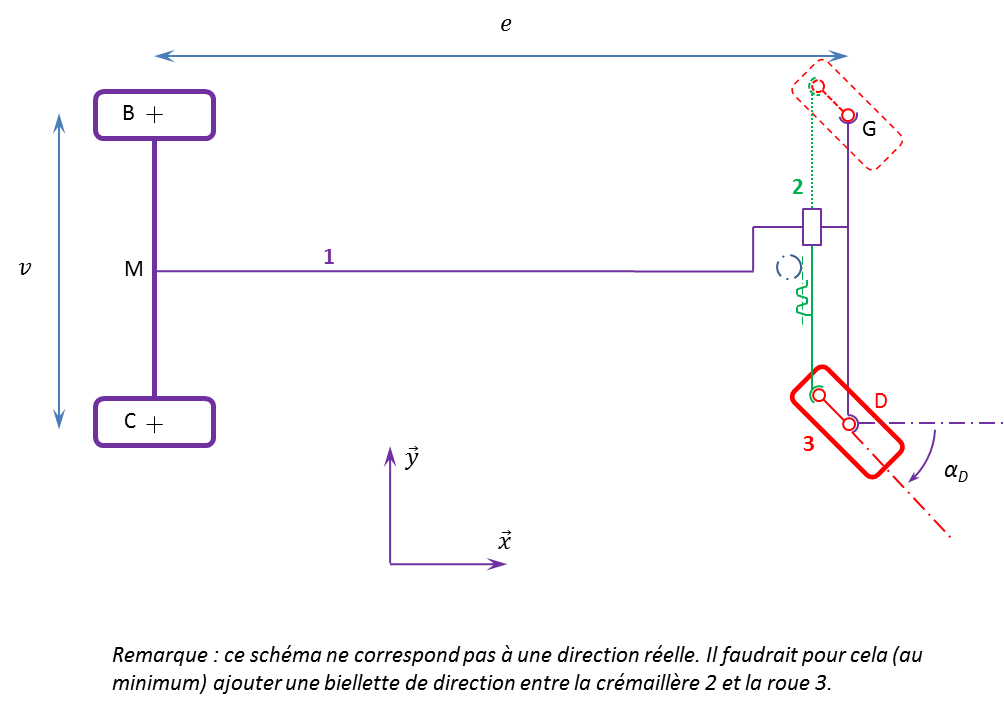
\includegraphics[width=.9\textwidth]{png/voiture}
\end{center}



\begin{center}
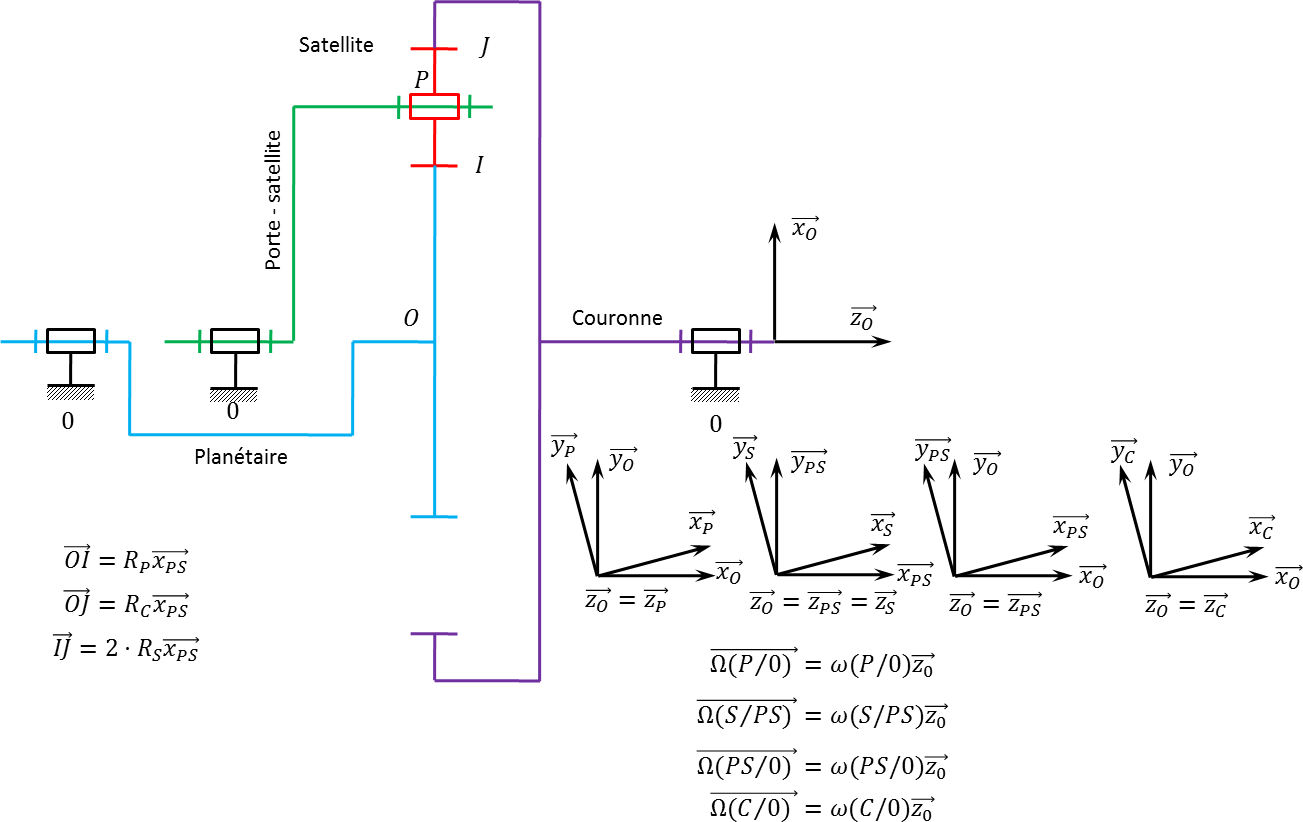
\includegraphics[width=.9\textwidth]{png/epi}
\end{center}


\section{Arbre d'appui}
Les dessin de définition est coté en utilisant le système de tolérances générales suivant : \textbf{ISO 2768 mK}. Vous vous référerez au TD sur le kart pour connaître les intervalles de tolérance associés. 

\paragraph{}
\textit{En utilisant le dessin de définition, interprétez les spécifications géométriques suivantes :}

\begin{center}
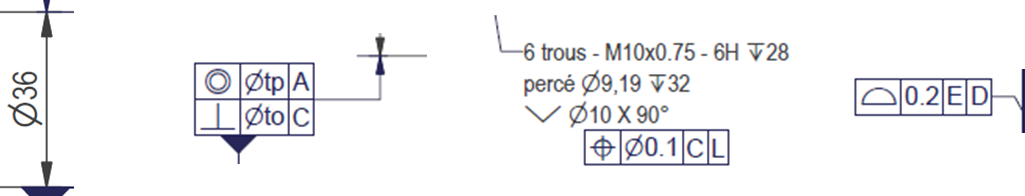
\includegraphics[width=.8\textwidth]{png/specif}
\end{center}
\end{document}
